\begin{definition}
A homogeneous function $f(x,y, z)$ is called a triangle center function (TCF) if $f(x, y, z)=f(x, z, y)$.
By homogeneous we mean $f(tx,ty,tz)=t^nf(x,y,z)$.
\end{definition}

For a given triangle center function, the trilinear $f(a,b,c):f(b,c,a):f(c,a,b)$ defined a unique point in the plane, we call it a
center. 
Two different triangle center functions can define the same triangle center. 
For example, $\frac1a$ and $bc$ both define the centroid. Two different trangle center functions define the same centers if and only 
if their ratios is a symmetric function of $a, b, c$.

Fermat point: the triangle center function is: $f(a,b,c)=\csc(A+\pi/3)$.


\begin{definition}
Given triangle $ABC$. For any point $P$ inside the triangle there are numbers $\lambda_1, \lambda_2, \lambda_3$
such that $\lambda_1+\lambda_2+\lambda_3=1$ and $\overrightarrow {OP}=\lambda_1\overrightarrow{OA}+\lambda_2\overrightarrow{OB}
+\lambda_3\overrightarrow{OC}$, $(\lambda_1, \lambda_2, \lambda_3)$ is called the barycentric coordinates.
\end{definition}


\begin{definition}[Cevian triangle]
Given triangle $ABC$, and a point $P$ inside $ABC$, $AP$ meets $BC$ at $D$, $BP$ meets $AC$ at $E$,
$CP$ meets at $AB$ at $F$. $\triangle DEF$ is called the {\bf Cevian triangle} of $\triangle ABC$ with respect to $P$.
\end{definition}


\begin{definition}[Anticevian triangle]
Given a triangle $ABC$, and a given $P$. If we can find triangle $A'B'C'$ such that $ABC$ is the Cevian triangle
of  $A'B'C'$ with respect to $P$, then we call $A'B'C'$ the anticevian triangle of $ABC$ with respect to $P$.

\end{definition}


\section{Isotomic conjugate}
Given triangle $ABC$, assume $M$ is the midpoint of $BC$. Given a poing $X$ on $BC$, assume $X'$ is the reflection of $X$ along
the center $M$, then $AX'$ is called the isotomic conjugate line of $AX$.


\begin{definition}
Given a point $P$ insider triangle $ABC$, assume $AP$ meets $BC$ at $X$, $BP$ meets $AC$ at $Y$, and $CP$ meets
$AB$ at $Z$; $AX', BY', CZ'$ are the isotomic conjugates of $AX, BY, CZ$, then $AX', BY', CZ'$ are concurrent.
\end{definition}
\begin{proof}
This follows immediately from Ceva's theorem.
\end{proof}

\begin{theorem}
Gergonne point and Nagal point are isotomic conjugates.
\end{theorem}

The proof is obvious.


\section{Symmedian}

\section{Generalized Cevian theorem}

I guess this theorem has been proved somewhere.
I believe it should be easy to prove:

\begin{theorem}
Given a triangle $ABC$ and any point $D$ on $BC$, $E$ on $AC$ and $F$ on $AB$, such that $\frac{AF}{FB}\cdot \frac{BD}{DC}\cdot \frac{CE}{EA}=1$,
the sign matters, then $AD, BE, CF$ are current.

\end{theorem}

Before proving this theorem, I want to give the motivation of this theorem.

\begin{theorem}
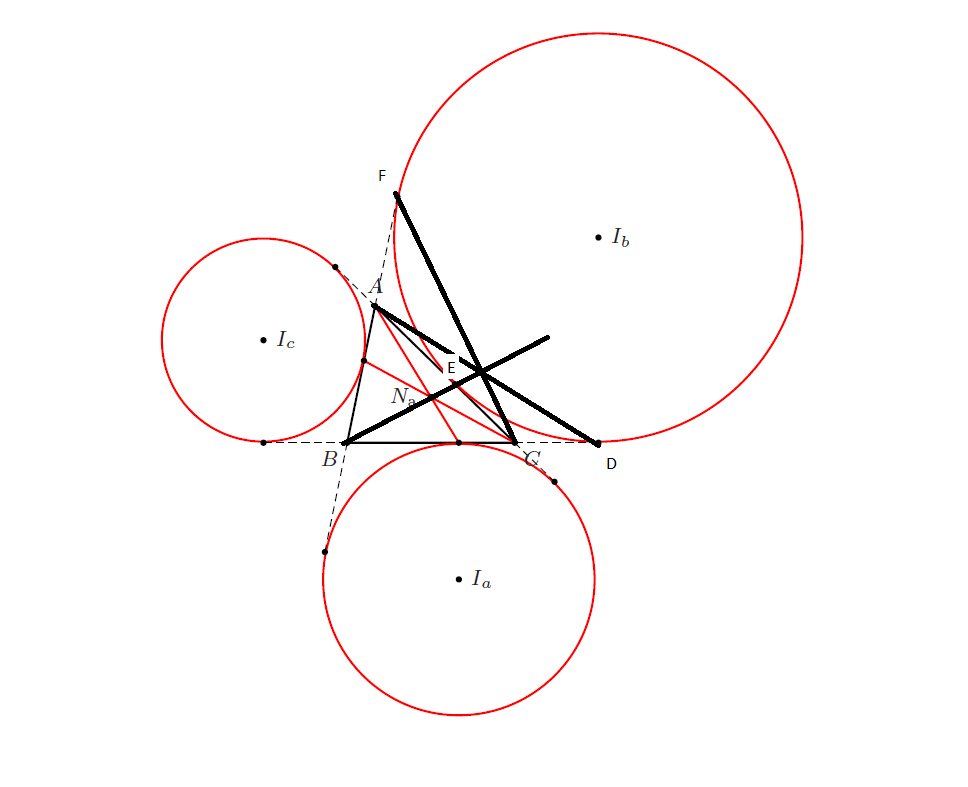
\includegraphics[width=3in]{excircle1.png}

If $D, E, F$ are the three tangents of the excircle to the three sides, then $AD, BE, CF$ are concurrent.
\end{theorem}

\begin{proof}
$AF=s-c, BF=s, BD=s, CD=s-a, CE=s-a, EA=s-c$, so the proof follows.
\end{proof}

I think this should be a 'known' center already, but I don't know yet.

\begin{theorem}
Assume the nine point circle tangents the three excircles at $D, E,F$ ($A$ corresponds to $D$), then
$AD, BE, CF$ are concurrent, this concurrent is called the second Feuerbach point. (which iis $X_{12}$)


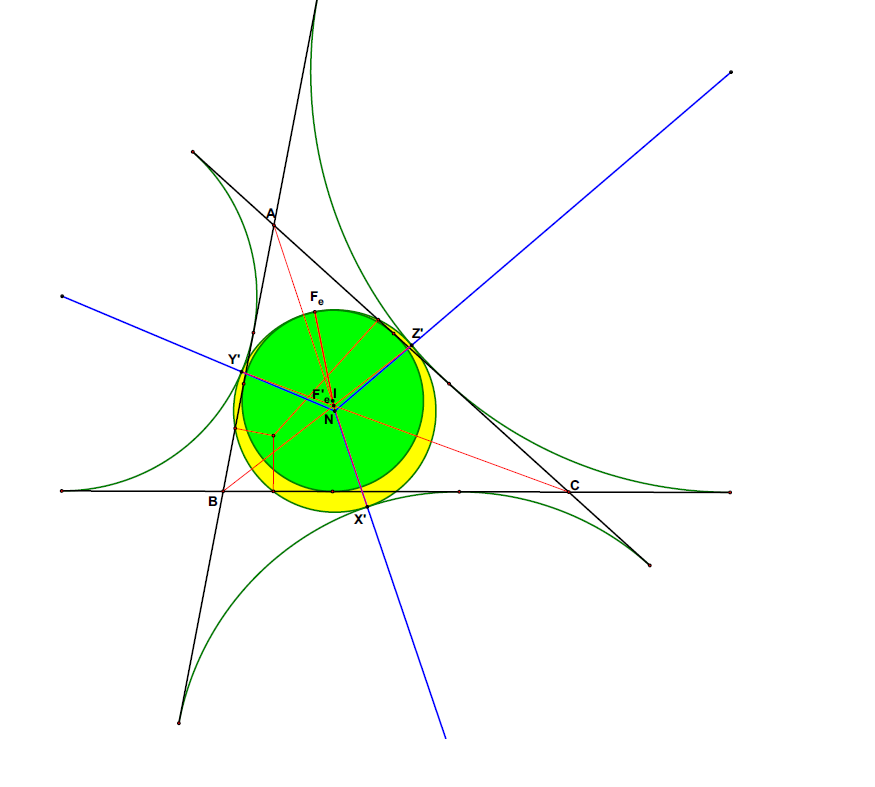
\includegraphics[width=3in]{excircle2.png}
\end{theorem}

\begin{theorem}
The symmedian point $K$ is the perspector of the reference triangle and the tangential triangle.
\end{theorem}

\begin{proof}
We had this proof already, but using the rule of sine to calculate the ratio and by the end to prove $AA'$ is a symmedian.

The following figure shows a better proof.


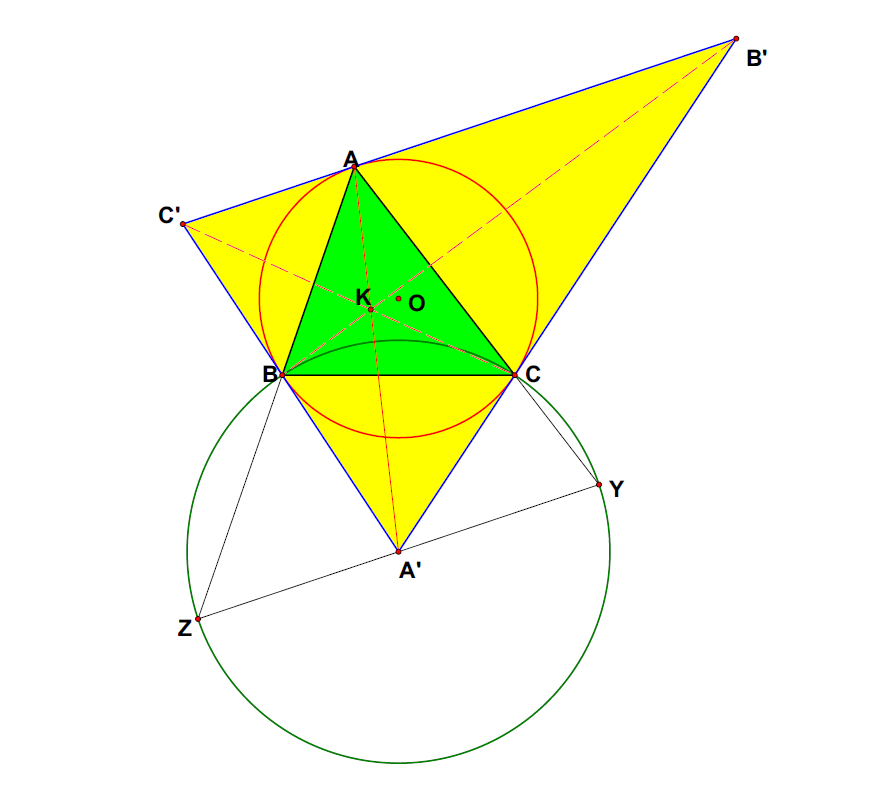
\includegraphics[width=3in]{tangentialcircle1.png}

I.e. Making a circle whihc takes $A'$ as the center and $A'B$ as the diameter. Then $BC$ is antiparallel to $ZY$, and
$AA'$ is the median, so it is the symmedian on $BC$.
\end{proof}

The circumcenter of the tangential triangle is a point on the Euler line (of the reference triangle), which is $X_{26}$.

The internal center of similitude of the circumcircle and incircle is $G_e^{*}$. (the isogonal conjugate of the Gergonne center). $X_{55}$

The external center of similitude of the circumcircle and incircle is $N_a^{*}$.(the isogonal conjugate of the Nagal point).$X_{56}$

Gergonne point and Nagal point are isotomic conjugate. This is very obvious.

The Simon line is very interesting, 

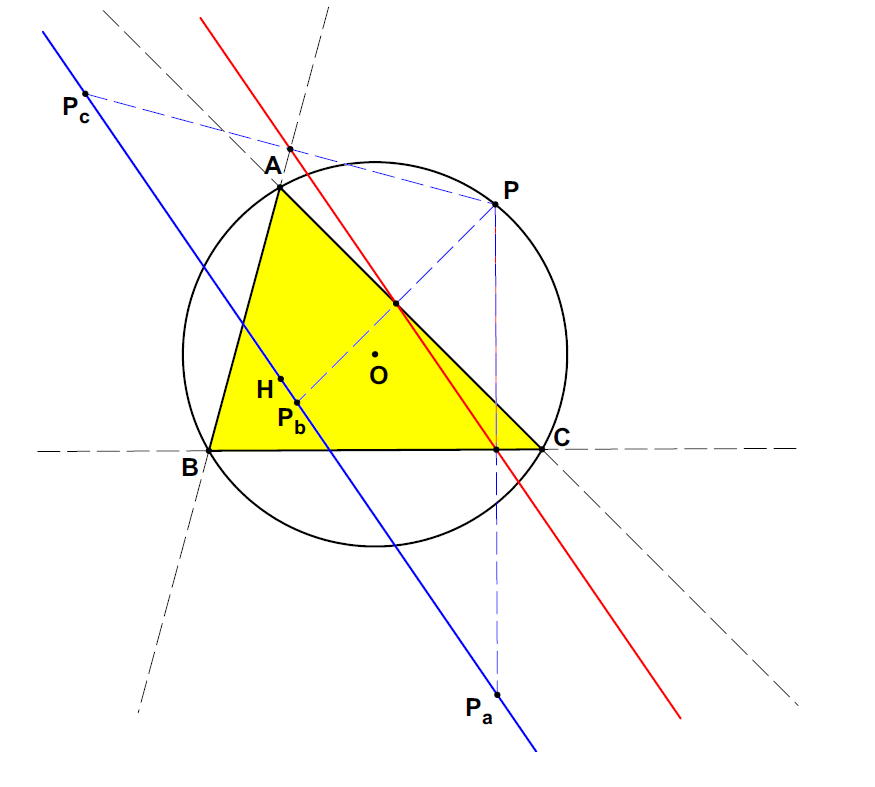
\includegraphics{simonline.png}

$P_c$ is the reflection point of $P$ about $AB$, similar to $P_b, P_c$. Then it is very easy to see that $P_a, P_b, P_c$ are collinear.

The very amazing thing is that $H$ is always on this line!!!

Also, the Simon line of antipodal points intersect orthogonally on the nine-point circle.

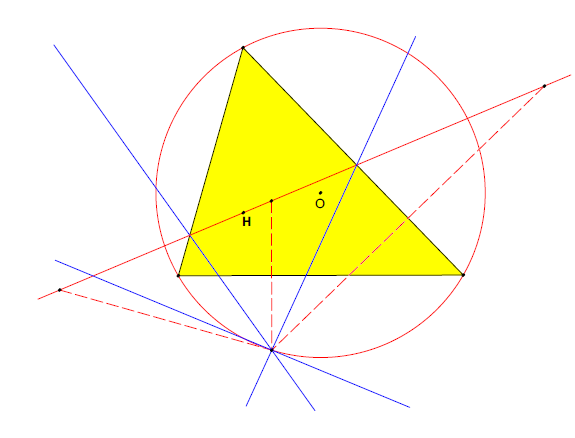
\includegraphics{simonline2}

Given any line $l$ passing $H$, then the reflection of $l$ about the three sides will meet at a point, which is the point will produce $l$ in
the above.

Especially, the Euler line will produce a point, called Euler relfection point? Which is $X_{110}$, also called Kiepert focus.

The following theorem is pretty amazing.

\begin{theorem}
Given triangle $ABC$, and makes triangle $BCX, CAY, ABZ$ upwards, assume $\angle X+\angle Y+\angle Z=180^\circ$,
then the circumcircles of $\triangle BCX, CAY, ABZ$ will meet at a point.

\end{theorem}

Especially if $YZ$ passes $A$, $XZ$ passes $B$ and $XY$ passes $C$, then it is true. (we already seen the following theorem:
\begin{theorem}
given a triangle $ABC$ and artrarily choose 3 points $D$ on $BC$, $E$ on $AC$ and $F$ on $AB$, the the circumcircles of
$\triangle AEF, BDF, CEF$ will meet at a point, so now it is clear).

\end{theorem}

\begin{theorem}
If $\triangle BCX, YAC, AZB$ are similar, then the theorem also hold.
\end{theorem}

\begin{theorem}

If $\triangle BCX, YAC, AZB$ are similar, let $P$ be the center of the circumcircle of $BCX$, $Q$ be
the center of the circumcircle of $YAC$, and $R$ be the center of the circumcircle of $AZB$.
Then $\triangle PQR\sim \triangle XBC$.
\end{theorem}

\begin{proof}
The proof is straighforward by using radical axis. It is easy to see that $PQ\bot $ the common chord of circles $P$ and $Q$,
$PR\bot $ the common chord of circles $P$ and $R$, assume the common intersection point is $S$, then
$\angle P = 180^\circ-\angle BSC=\angle X$, similary for other angles, and the proof follows.
\end{proof}

This theorem immediately has a corollary, if all the upwards triangles are equilateral triangles, then
the centers form an equilateral triangle. This is so called Napeloen triangle.

Napeloen center is not Fermat center, but they all use the upwards equilateral triangles.

Let's talk about theorem 7 a little bit more. This theorem is true, even $D, E, F$ are collinear!
In this case, $A, E, C$ are such three points to $\triangle FBD$, so the circumcircles of $\triangle DEC, BAC, FAE$
will meet at a point. The theorem above say the circumcircles of $\triangle AEF, BDF, CED$ will meet at a point.

So they all passes the intersection point of the circumcircles of $\triangle AEF$ and $CDE$, so those 4 circles
meet at a point. This is pretty amazing.

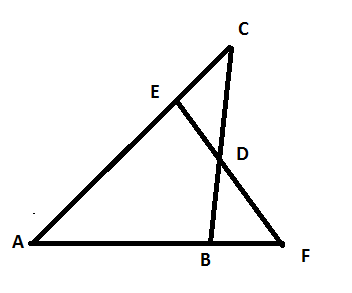
\includegraphics[width=2in]{theorem9}

\begin{theorem}
In the figure above, the circumcircles of $\triangle AEF, BDF, CED, ABC$ will meet at a point.
\end{theorem}

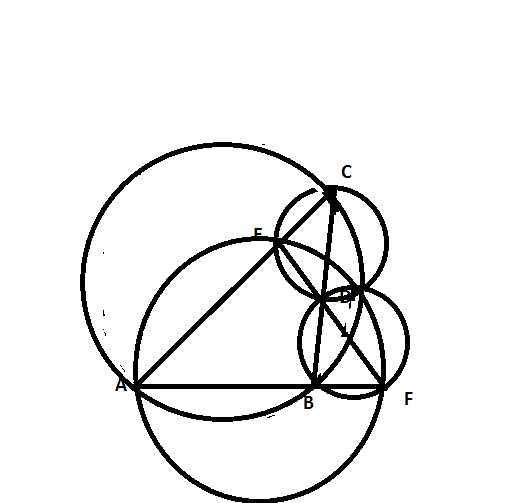
\includegraphics[width=2in]{theorem10}


Assume those 4 circles intersect at a point $P$, 
assume $AP(AEF), BP(BDF), CP(CDE)$ are the diameters, then $PD\bot BC, PE\bot AC, PF\bot AB$, 
which means $DEF$ is the Simon line.